\documentclass[hidelinks,12pt]{article}
\usepackage[utf8]{inputenc}
\usepackage[T1]{fontenc}
%\usepackage[french]{babel}
\usepackage{times}
\usepackage{hyperref}
\usepackage{graphicx}
\usepackage{caption,graphicx,enumitem}
%\usepackage{titlesec}

%\setcounter{secnumdepth}{4}


\begin{document}

\title{Research project report}
\author{Bastien Nony, Alban Gossard\\
Institut National des Sciences Appliquées,\\
Toulouse,\\
\href{mailto:nony@etud.insa-toulouse.fr}{   \texttt{nony@etud.insa-toulouse.fr}}\\
\href{mailto:gossard@etud.insa-toulouse.fr}{   \texttt{gossard@etud.insa-toulouse.fr}}}
\date{\today}

\maketitle

\begin{abstract}
In this work we study surrogates problems for different types of modelling problem. The objective is to provide fast calculation for undetermined values. Beginning from physical equations such as Saint-Venant's, we add statistical formulas to determine the variability of the system. This study registers in the frame of geostatistics.
\end{abstract}

\newpage

\tableofcontents



\section{Objectives}
\section{Key notions}


\section{Interpolation par krigeage}

Calculer toutes les valeurs est temporellement impossible. Supposons que l'on veuille déterminer la réparitition de la densité de charbon sur chaque mètre carré de la région Lorraine, la tâche serait longue et fasitidieuse. Chaque relevé coûterait du temps et de l'argent et serait surtout inutile. Plutôt que d'effectuer nos mesures sur chaque mètre carré, on se propose d'effectuer des mesures tous les 500 mètres et d'ensuite relier les données sur l'ensemble du territoire. Cette façon de procéder conduit à la notion d'interpolation.

Une première idée serait d'interpoler de manière déterministe par interpolation linéaire, polynomiale, etc. Cette méthode pose plusieurs problèmes. Il sera impossible par formalisme mathématique de quantifier l'incertitude. En effet, les variables déterministes ne permettent pas d'estimer des variations potentielles/non prévisibles. Pour cette raison principalement une alternative propose une interpolation stochastique. Plusieurs méthodes peuvent être proposées : krigeage, polynômes du chaos.

Introduisons quelques outils statistiques :

\subsection{Variogramme}





\subsection{Interpolation par krigeage}

Cette méthode est probablement la plus évidente relativement au formalisme mathématique. Il s'agit d'une estimation linéaire où chaque estimation se fera linéairement en fonction de valeurs exactes mesurées au environs et associées à des poids particuliers.

Ainsi, la procédure est la suivante :

(1) On délimite notre zone d'étude en intervalles de paramétrage.

(2) On mesure, calcule à partir d'un modèle physique de départs un certain nombre de données idéales (X_1,$\ldots$,X_n)

(3) Pour un certain point donné dans notre espace délimité on trouve l'estimateur associé en calculant la matrice de poids correspondante.
(4) notre estimateur en ce point vaut donc la somme des valeurs idéales * leur poids estimé correspondant

Mathématiquement cela donne :

(1) pour un krigeage simple




(2) Pour un krigeage ordinaire

Cette approche apporte plusieurs avantages :


Tout d'abord il est possible de quantifier la variance de notre estimation par le biais de la variance du krigeage :



Les poids de krigeage adoptent des caractéristiques logiques :

(1)A l'infini les points n'apportent plus d'information sur le résultat

(2) Si le nombre de valeurs dans une région donnée est grand alors les poids sont très faibles. Cela s'explique par le fait que chaque point influe davantage sur les zones qui lui sont très proches et moins sur les zones lointaines où l'information se partage entre beaucoup de données.

(3) Dans les régions où il y a peu de données, le krigeage reflète une estimation de la moyenne.

\section{Interpolation par polynomes du chaos}


%%Comment choisir les points de référence? Méthode quasi aléatoires
\section{}


\section{Study of 1D model}
\subsection{Presentation}
\subsection{Theoretical tools}
\subsection{Surrogate model analysis}
\subsubsection{First example : Ishigami}
\subsubsection{Garonne Model }

\paragraph{Surrogate method : kriging}
\hspace{1cm}

We compute different surrogate using different initial sample size. These surrogates were computed using a least square strategy. Figure \ref{influence_init_size_method_surrogate_kriging} gives the simulations results for the surrogate. One can observe that we obtain almost the same resultats as the initial sample size is greater than 10. As we will explain in part \ref{}, the results are quite precise but we have no information about the standard deviation of this new model and its sensibility to the parameters. Computing a surrogate with a greater number of points is fundamental to get a quantification of the error.

\begin{figure}
  \centering
  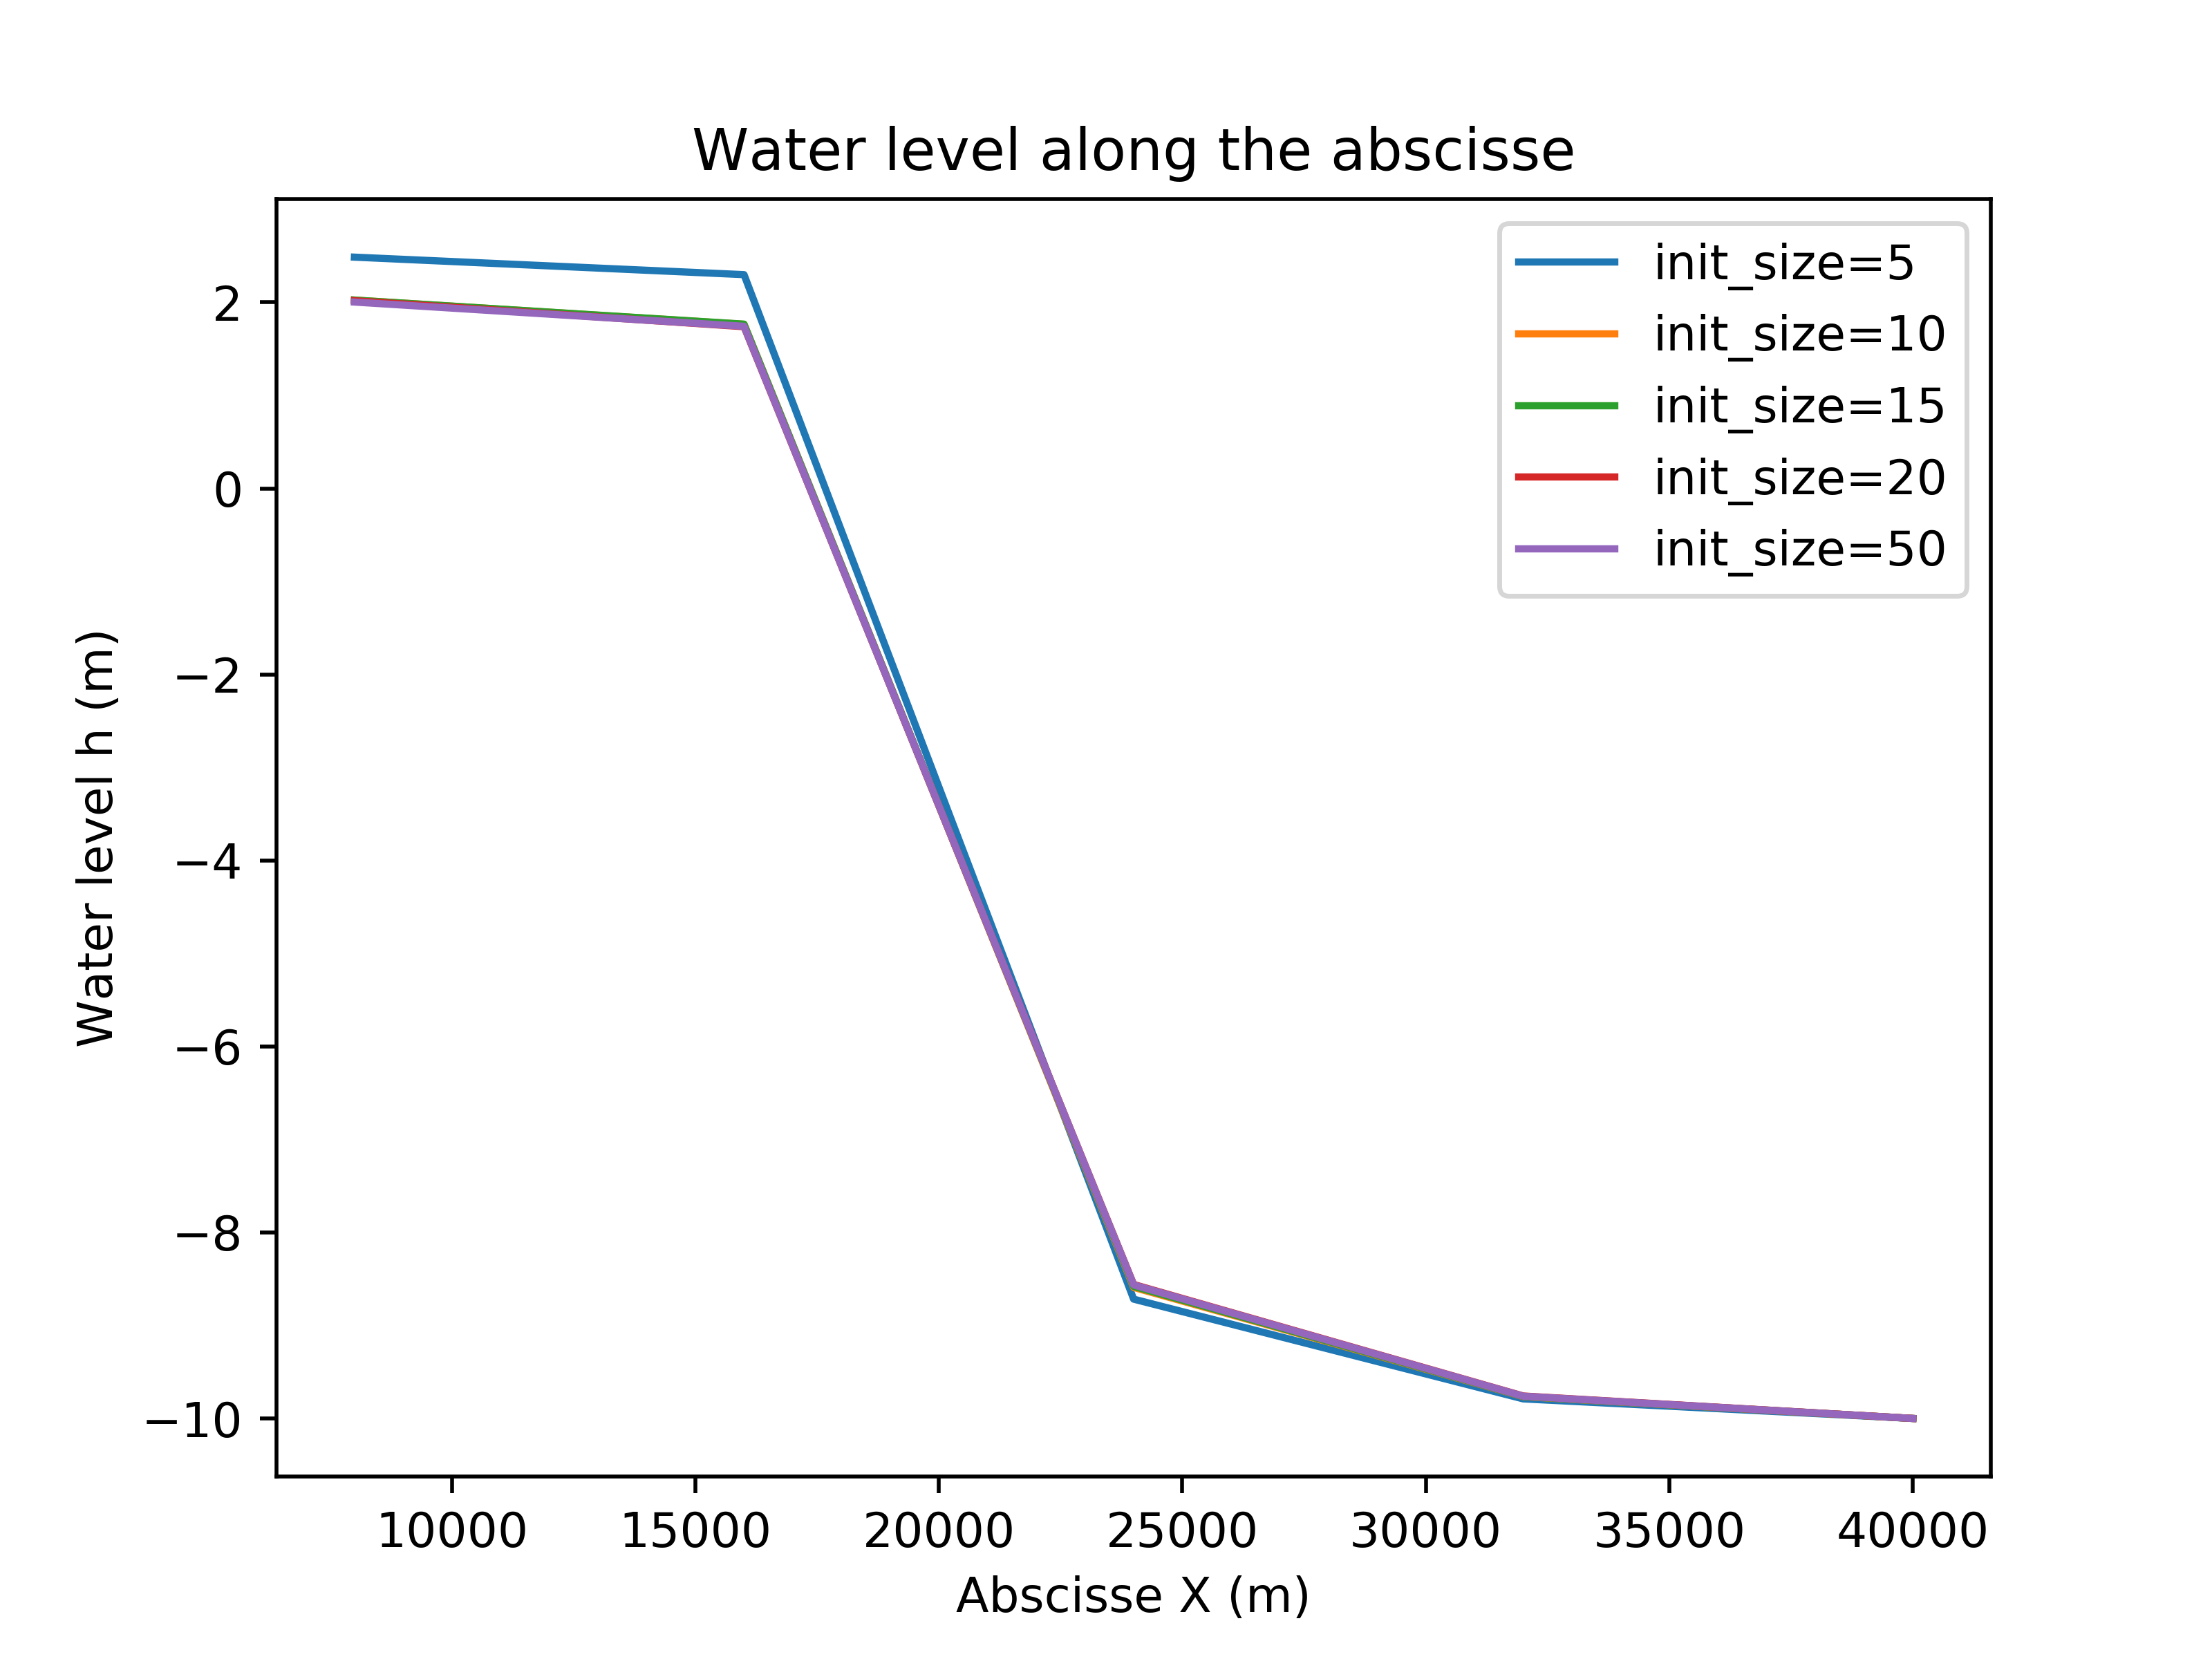
\includegraphics[width=0.8\textwidth]{images/influence_init_size_method_surrogate_kriging.png}
  \caption{Water level along the abscisse for simulations with different initial sample size using kriging method for surrogate computing.}
  	\label{influence_init_size_method_surrogate_kriging}
\end{figure}

\paragraph{Surrogate method : pc}
\hspace{1cm}

\begin{figure}
  \centering
  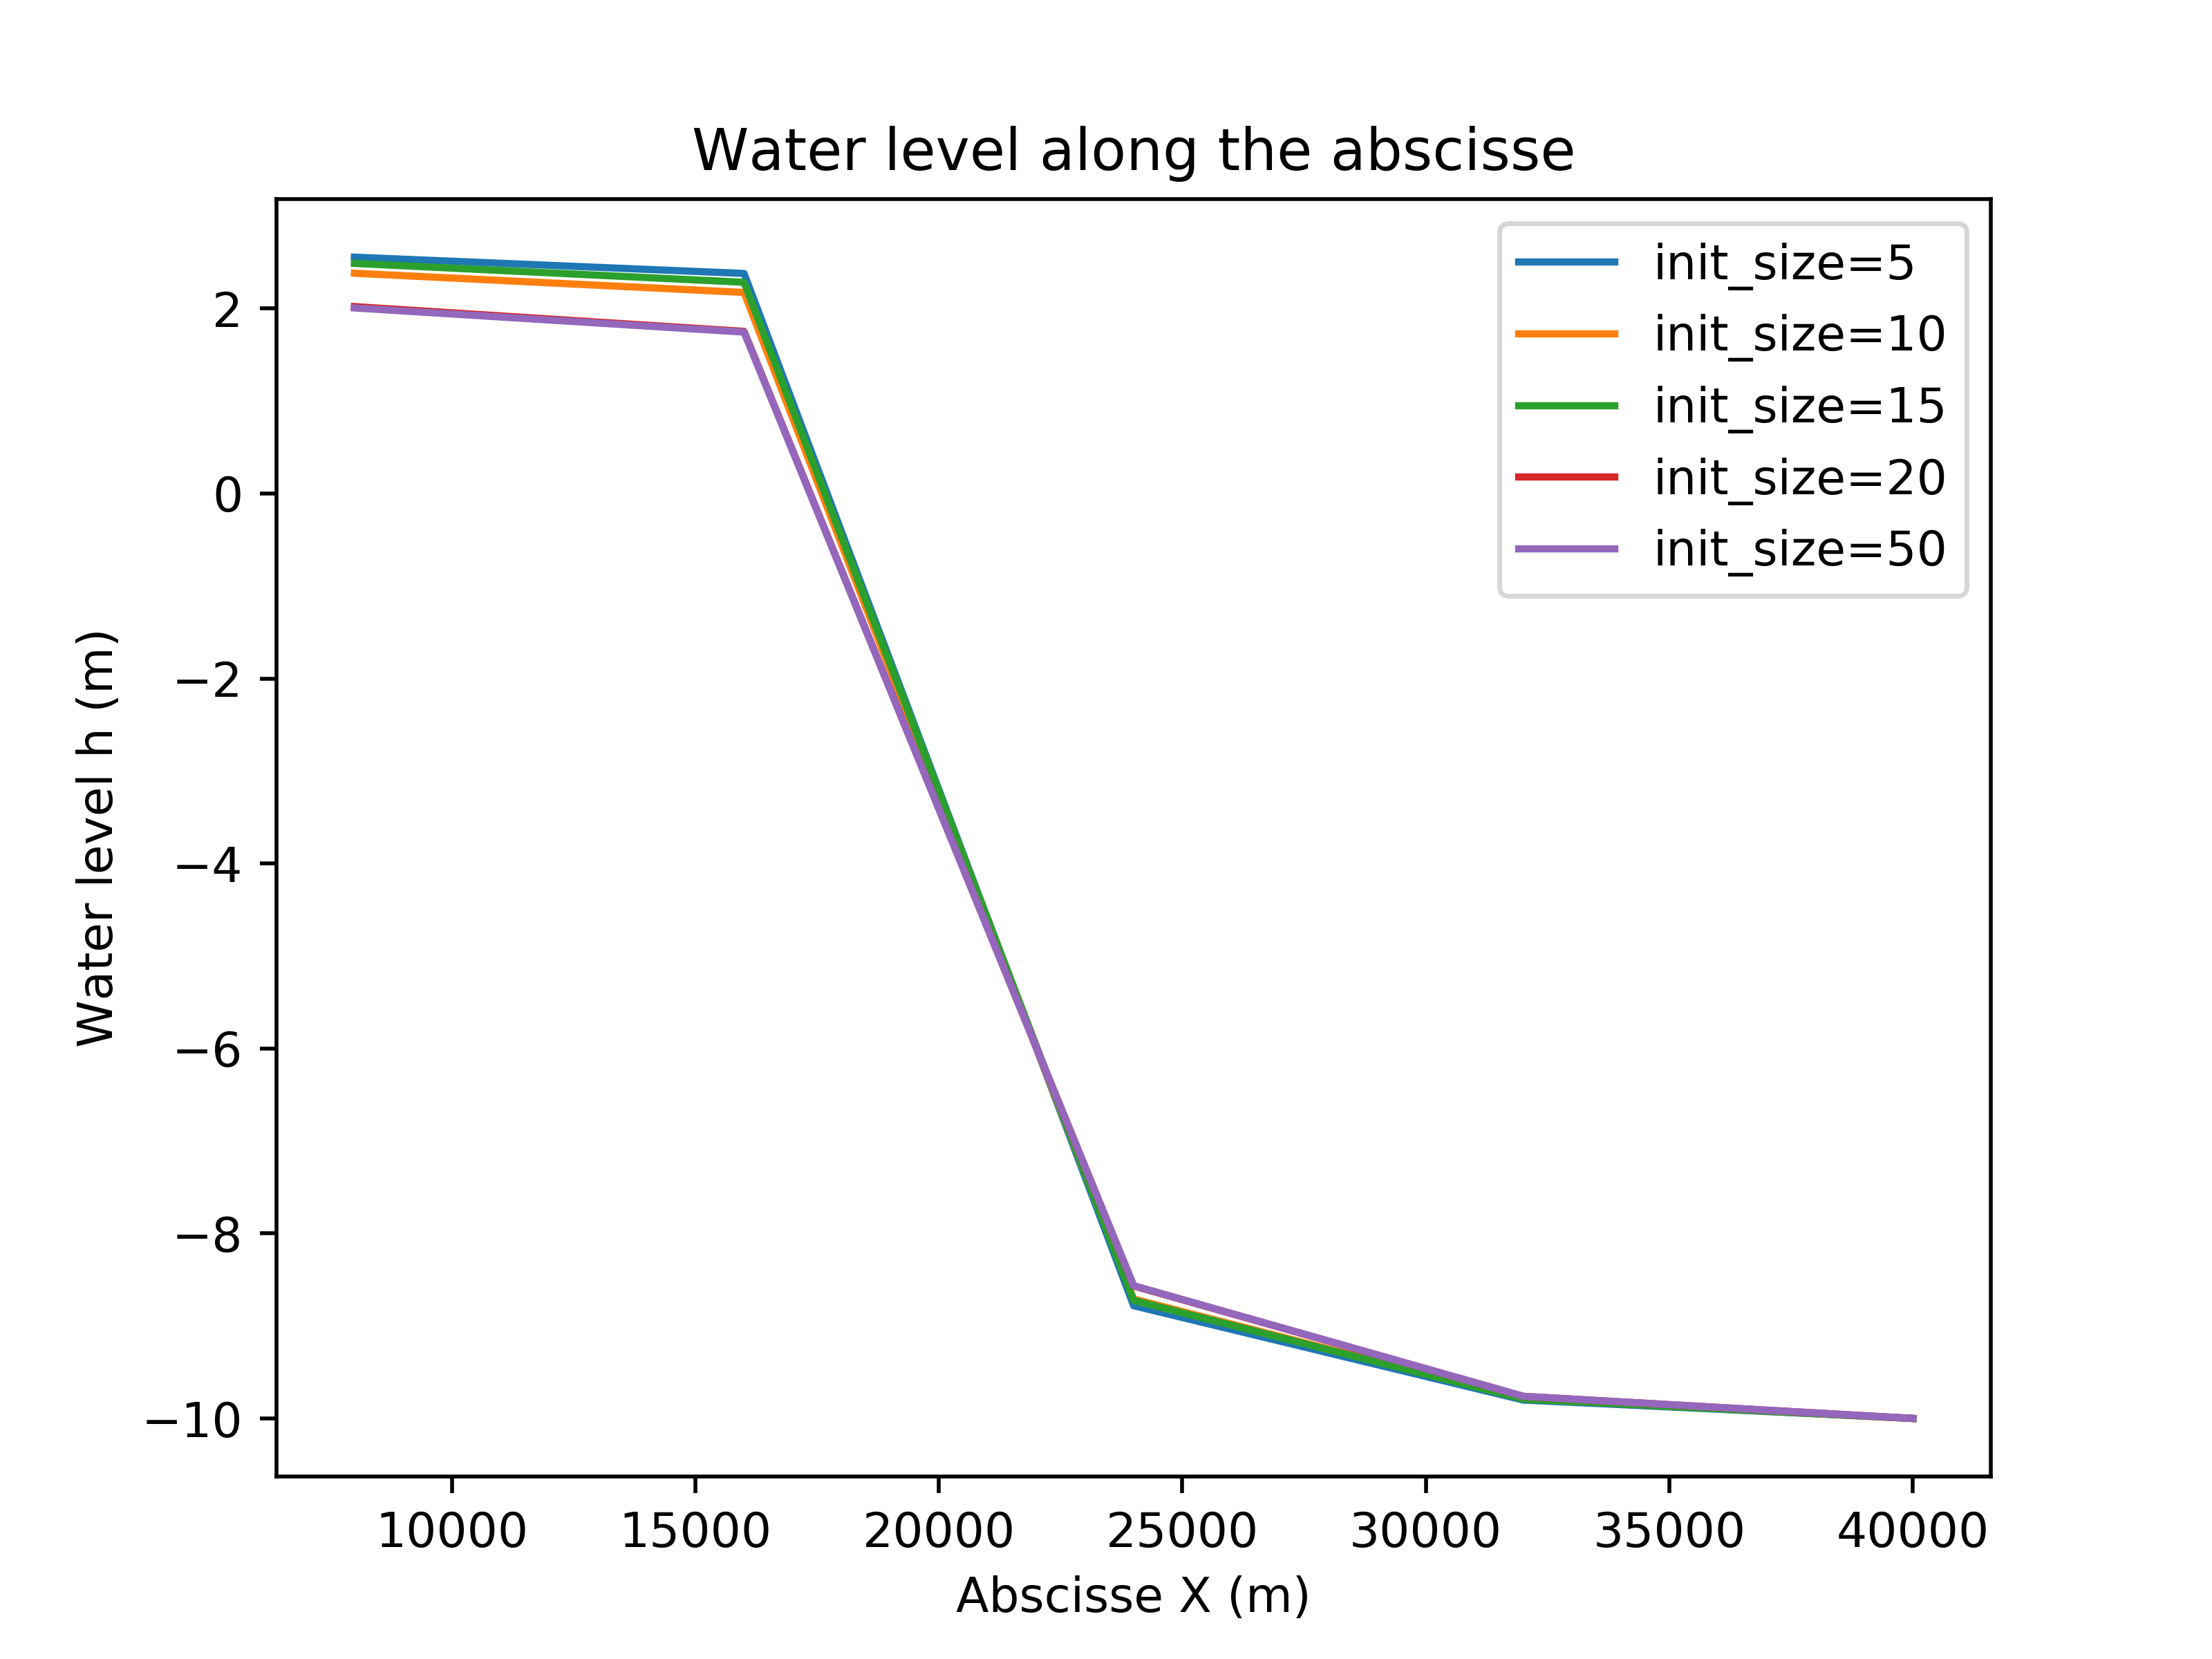
\includegraphics[width=0.8\textwidth]{images/influence_init_size_method_surrogate_pc.png}
  \caption{Water level along the abscisse for simulations with different initial sample size using pc method for surrogate computing.}
  	\label{influence_init_size_method_surrogate_pc}
\end{figure}

\begin{figure}
  \centering
  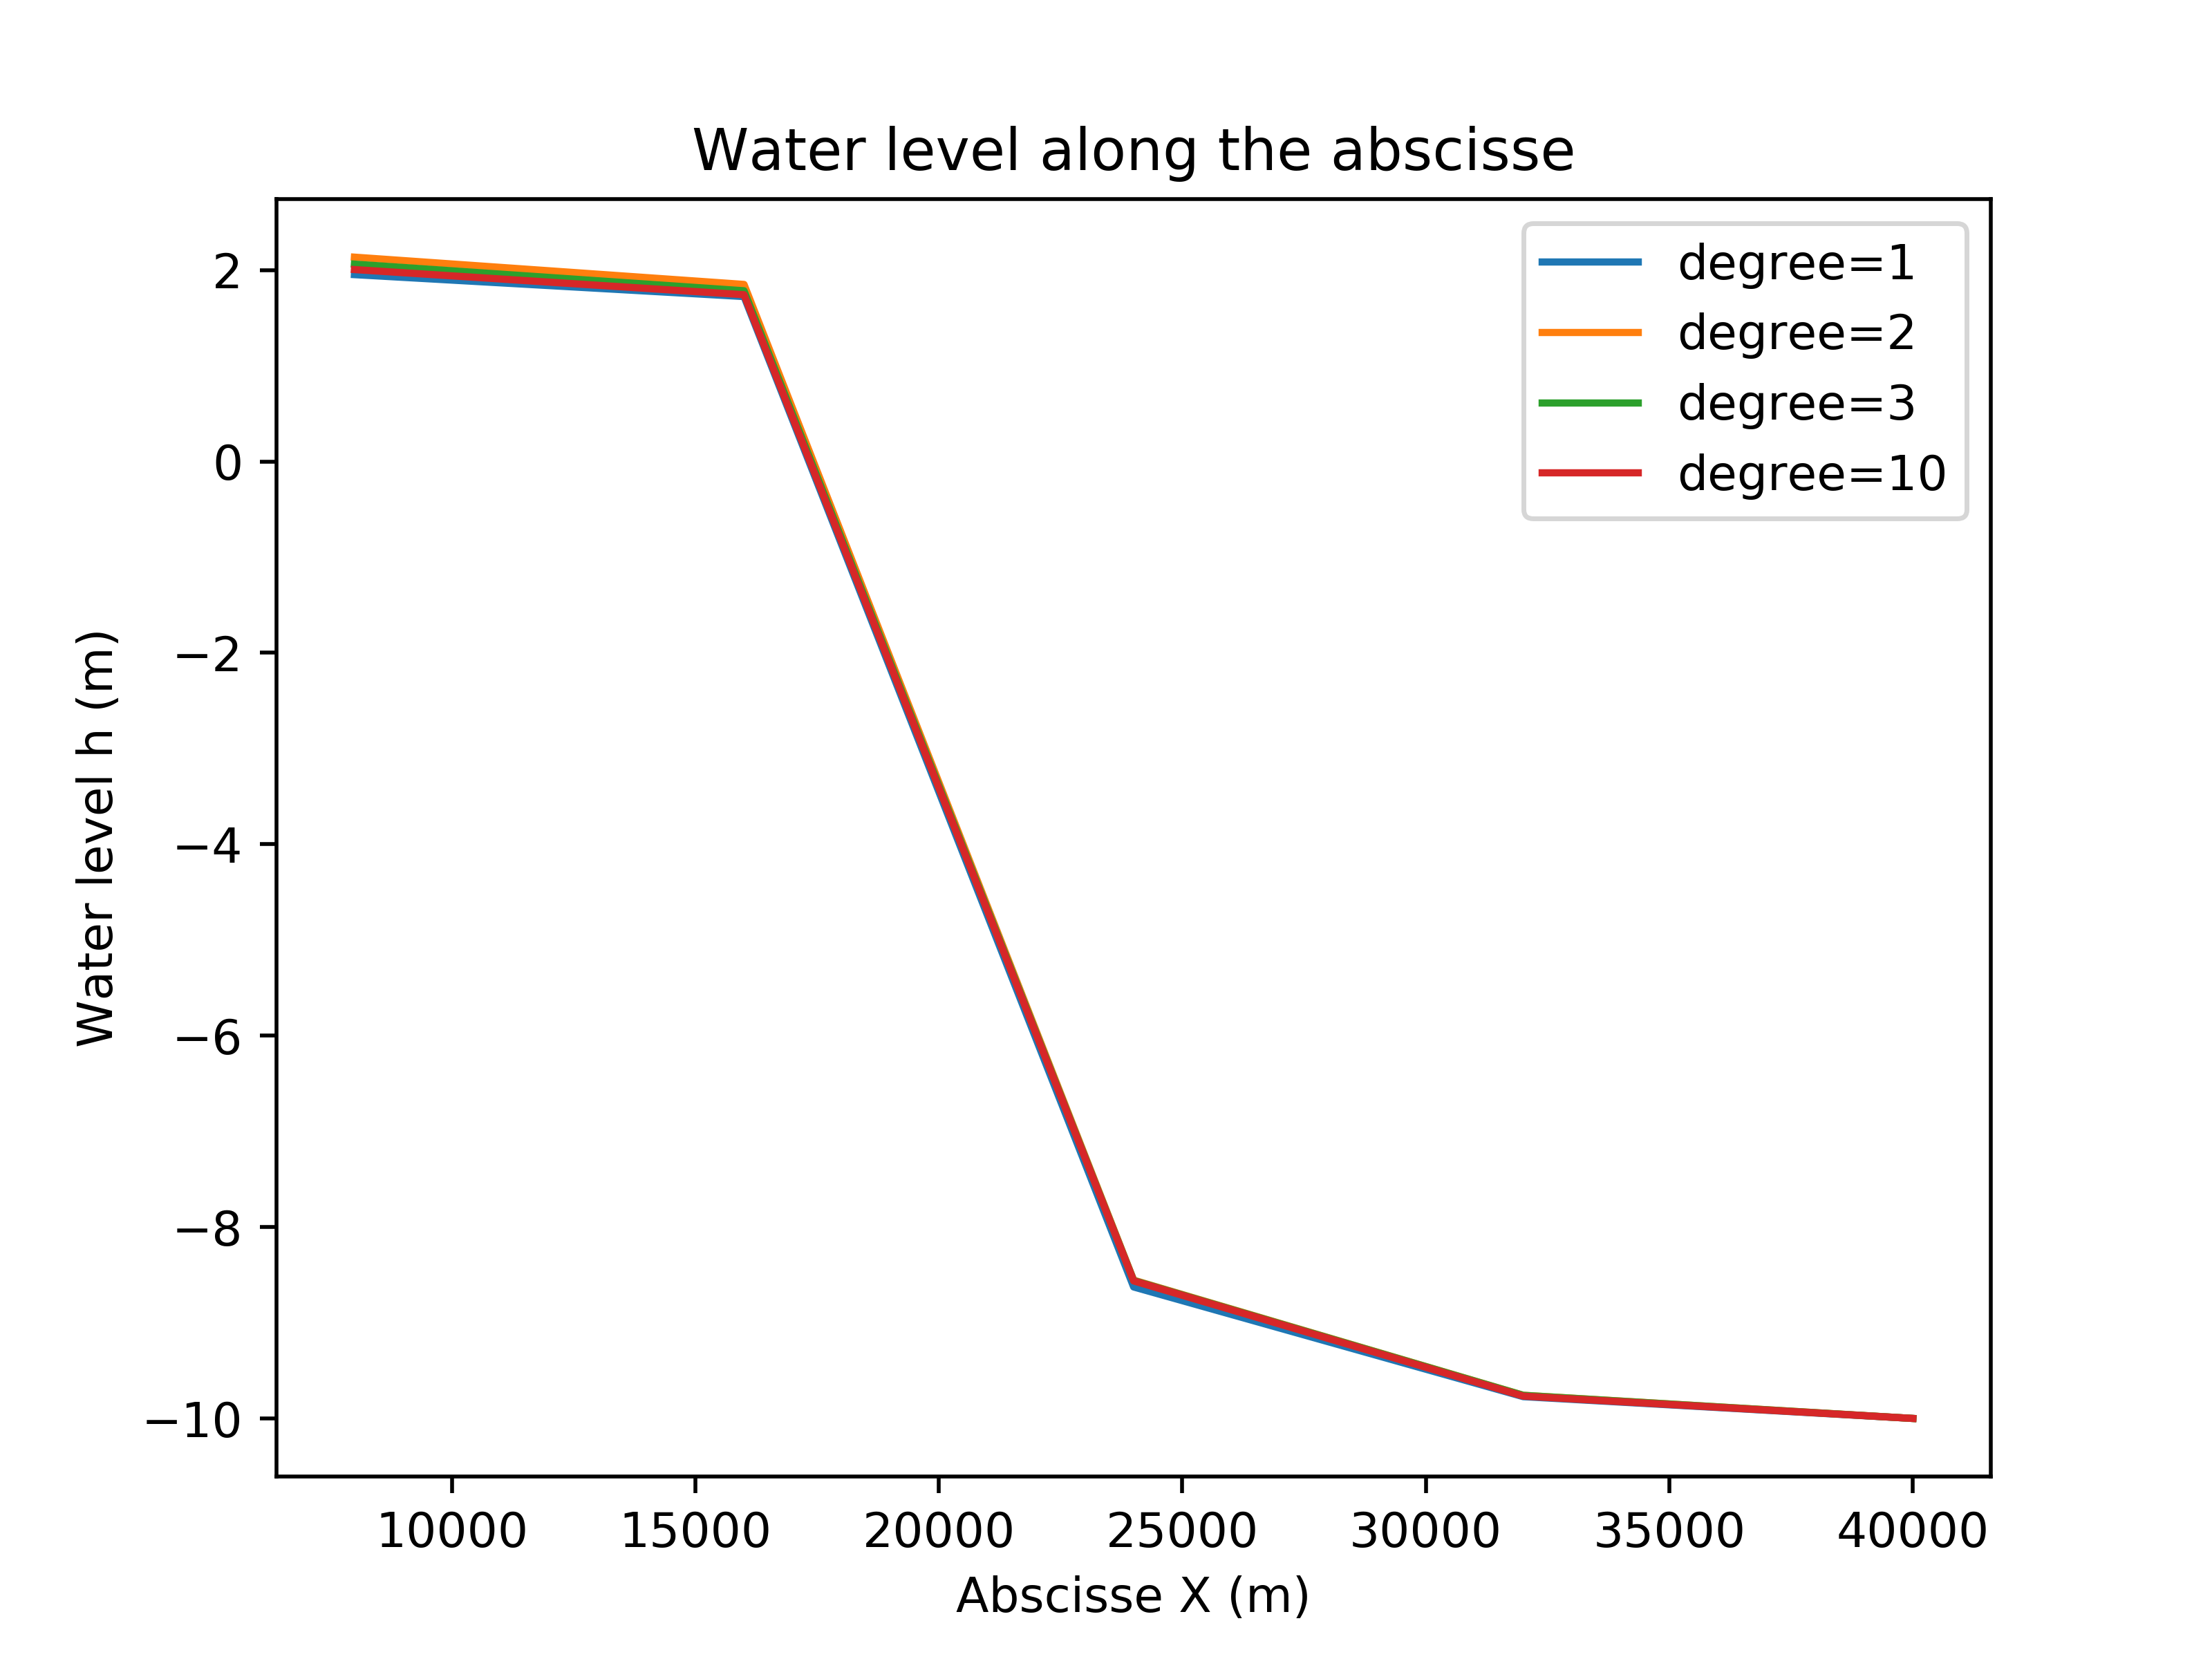
\includegraphics[width=0.8\textwidth]{images/influence_degree_method_surrogate_pc.png}
  \caption{Water level along the abscisse for simulations with different maximum pc degree.}
  	\label{influence_degree_method_surrogate_pc}
\end{figure}

\paragraph{Q2 study}
\hspace{1cm}

\begin{table}
\begin{tabular}{|c|c|}
  \hline
  Max pc degree & Q2 value \\
  \hline
  1 & 0.77805266\\
  2 & 0.95102133\\
  3 & 0.99238156\\
  4 & 0.99782457\\
  5 & 0.99813309\\
  \hline
\end{tabular}
\caption{Q2 value for different maximum pc degree using pc method for surrogate computing.}
\label{influence_degree_method_surrogate_pc_Q2}
\end{table}

\subparagraph{Distributions}
\hspace{1cm}

\begin{figure}
  \centering
  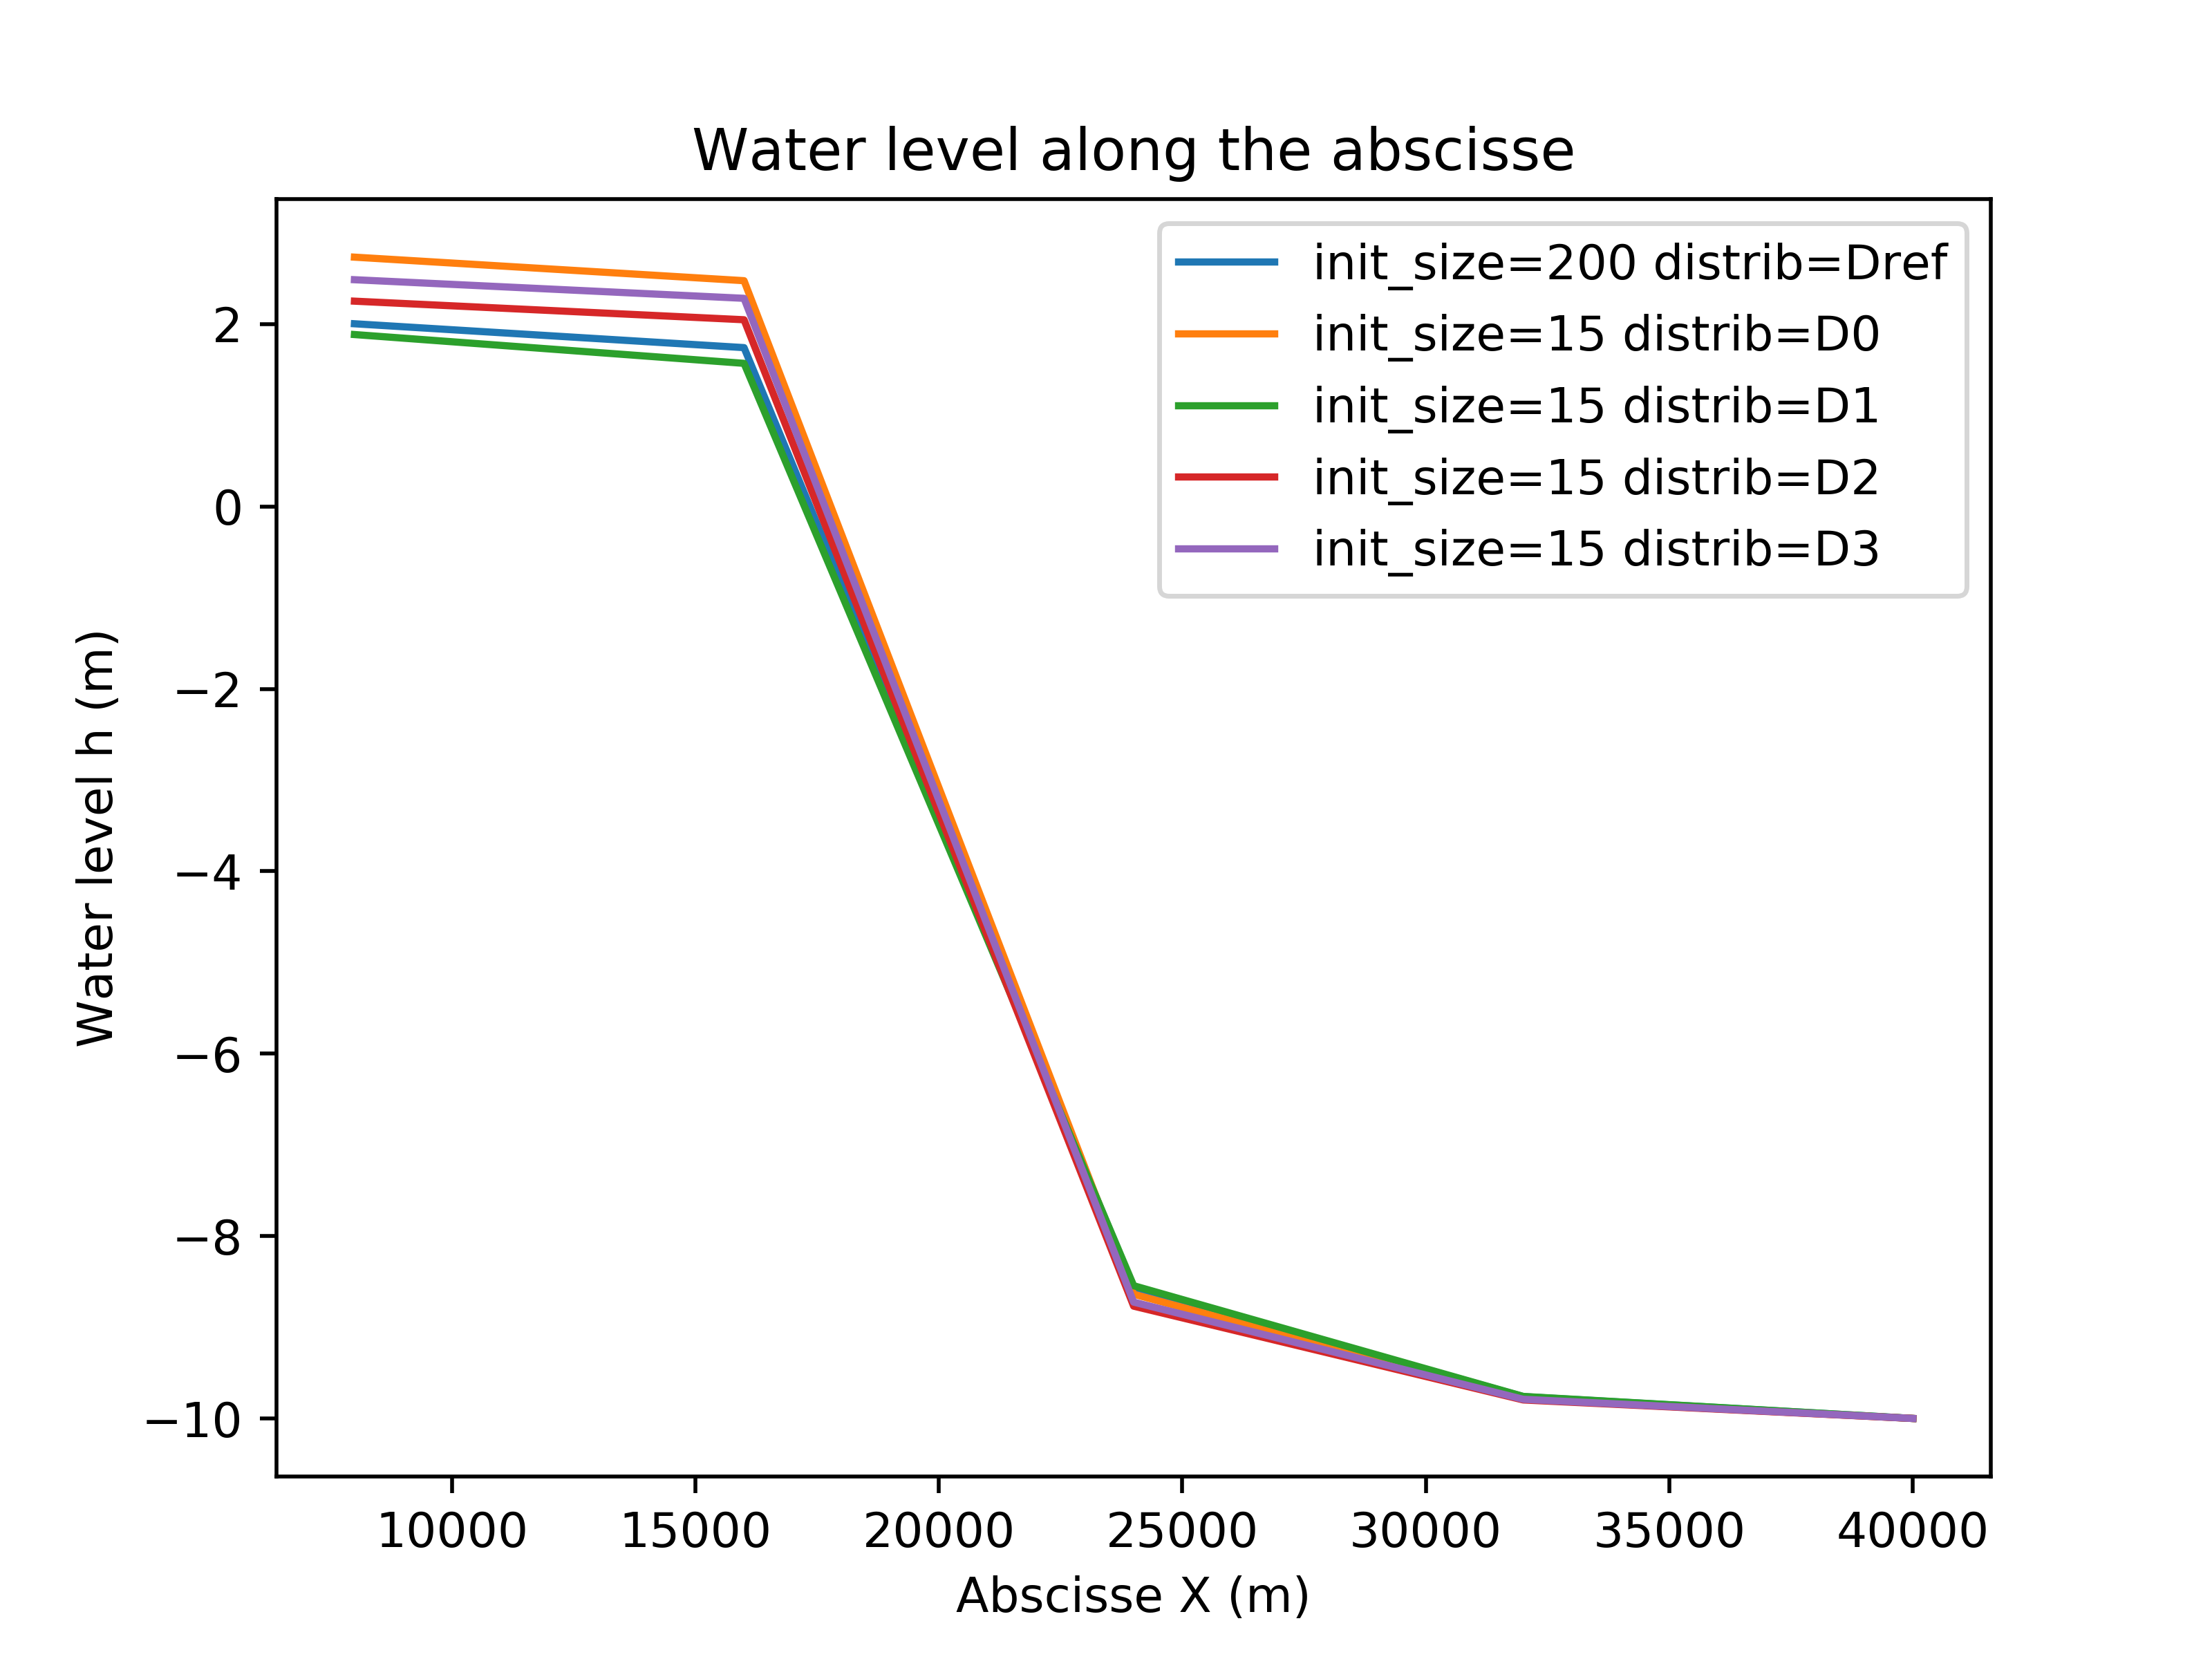
\includegraphics[width=0.8\textwidth]{images/influence_distributions_least_square.png}
  \captionsetup{singlelinecheck=off}
  \caption[]{Water level along the abscisse for simulations with different distributions for $Q$ and $K_s$ using least square strategy for surrogate computing. Distributions are the following : \begin{itemize}
  \item $D_{ref}$ : $K_s\sim BetaMuSigma(37.5, 5, 15, 60)$, $Q\sim BetaMuSigma(4035, 400, 2500, 6000)$
  \item $D_0$ : $K_s\sim Uniform(15, 60)$, $Q\sim Uniform(2500, 6000)$
  \item $D_1$ : $K_s\sim Uniform(15, 60)$, $Q\sim BetaMuSigma(4035, 400, 2500, 6000)$
  \item $D_2$ : $K_s\sim BetaMuSigma(37.5, 5, 15, 60)$, $Q\sim Uniform(2500, 6000.)$
  \item $D_3$ : $K_s\sim BetaMuSigma(37.5, 5, 15, 60)$, $Q\sim BetaMuSigma(4035, 400, 2500, 6000)$
  \end{itemize}}
  	\label{influence_distributions_least_square}
\end{figure}

One can consider that the $D_{ref}$ distribution is a good approximation of real $Q$ and $K_s$ values, meaning that we can compare different distributions with an initial sample size small to $D_{ref}$ distribution (which is computed with a high initial sample size). Figure \ref{influence_distributions_least_square} gives water level along abscisse for different sampling distributions on $Q$ and $K_s$. The distribution $D_1$ is the closest one to $D_{ref}$ suggesting we should sample the space $(Q,K_s)$ using a uniform distribution on $K_s$ and a normal one on $Q$.

\subsubsection{Michalewicz example}





%\section{Annex}

%\subsection{Polynomial Chaos} ?????




\end{document}
